\documentclass{article}
\usepackage[utf8]{inputenc}
\usepackage{amsmath}
\usepackage{graphicx}
\usepackage{geometry}
\graphicspath{{images/} 
\geometry{legalpaper, lmargin=0.7in, bmargin=1in}}

\begin{document}
\newpage

\section{Développment Chebychev}

\subsection{Contraintes}
Selon le diagramme de contraintes suivant,
\begin{center}
	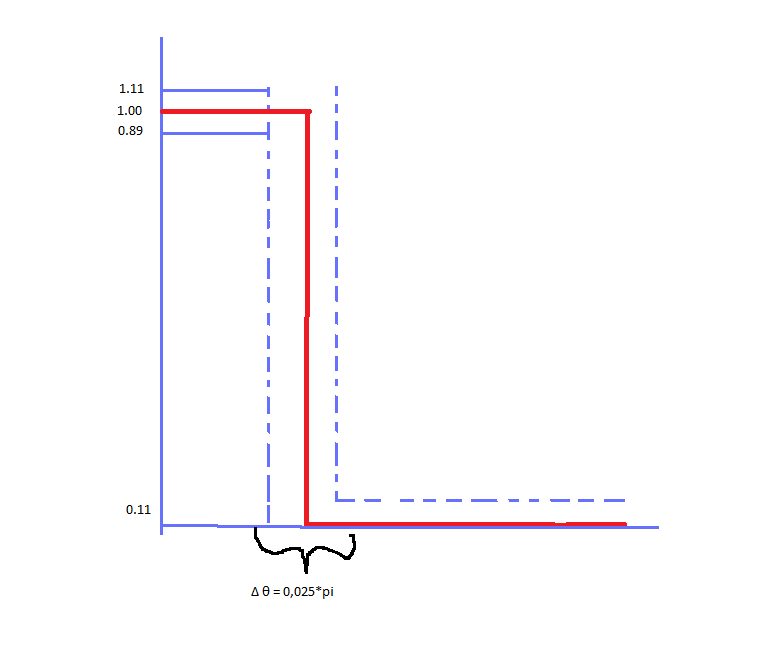
\includegraphics[width=\textwidth]{DiagrammDeContrasadaser}
\end{center}

Nous déterminons $\delta_1 = 0.11$, $\theta_p = 0.1\pi$ et $\theta_s = 0.15\pi$ en fréquence normalisée $Fe = 1$.
\newline
\subsection{Gauchissement}
Par la suite, il faut faire le gauchissement des angles $\theta$,
\newline
\begin{equation}
\omega = 2 \times Fe \times \tan(\frac{\theta}{2})
\end{equation}
\begin{equation}
\omega_p = 2 \times Fe \times \tan(\frac{\theta_p}{2}) = 0,3168
\end{equation}
\begin{equation}
\omega_s = 2 \times Fe \times \tan(\frac{\theta_s}{2}) = 0,4802
\end{equation}
\subsection{Trouver les pôles et les zéros selon l'angle}
Par la suite, il faut trouver les pôles et les zéros du filtre,
\begin{equation}
\phi_k = \frac{\pi}{2} + \frac{\pi \times (2*k+1)}{2}
\end{equation}
Puisqu'on s'est imposé un filtre d'ordre 1,
\begin{equation}
N = 1
\end{equation}
Donc,
\begin{equation}
k = N - 1
\end{equation}
\begin{equation}
k = 0
\end{equation}
Ensuite,
\begin{equation}
\phi_k = \frac{\pi}{2} + \frac{\pi \times (1)}{2} = \pi
\end{equation}
\newline
Par la suite, il faut trouver $\epsilon^2$,
\begin{equation}
\epsilon^2 = \frac{1}{(1-\delta_1)^2}-1
\end{equation}
\begin{equation}
\epsilon^2 = \frac{1}{(1-0,11)^2}-1 = 0,2624
\end{equation}
Ensuite, il faut trouver $\beta$,
\begin{equation}
\beta = \frac{\sqrt[2]{1+\epsilon^2} + 1}{\epsilon}
\end{equation}
\begin{equation}
\beta = \frac{\sqrt[2]{1+0,2624} + 1}{0,5123}=4,1451
\end{equation}
Maintenant, il faut trouver les rayons des ellipses $r_1$ et $r_2$,
\begin{equation}
r_1 = \omega_p \times \frac{\beta^2 + 1}{2 \times \beta}
\end{equation}
\begin{equation}
r_1 = 0,3168 \times \frac{4,1451^2 + 1}{2 \times 4,1451} = 0,6947
\end{equation}
\begin{equation}
r_2 = \omega_p \times \frac{\beta^2 - 1}{2 \times \beta}
\end{equation}
\begin{equation}
r_2 = 0,3168 \times \frac{4,1451^2 - 1}{2 \times 4,1451} = 0,6183
\end{equation}
\newline
Pour trouver les zéros,
\begin{equation}
z_k = \infty
\end{equation}
Puisqu'il s'agit un Chebyshev 1, il y a une infinité de zéros.
\newline
\newline
Pour trouver les pôles,
\begin{equation}
p_k = r_2 \times cos(\phi_k) + j \times r_1 \times sin(\phi_k)
\end{equation}
\begin{equation}
p_0 = r_2 = 0,6183
\end{equation}
\newline
Car $sin(\pi) = 0$ et $cos(\pi) = 1$
\newline
\newline
Donc, la fonction de transfert du filtre analogique est,
\begin{equation}
H(s) = \frac{K}{s+0,6183}
\end{equation}
Sachant que,
\begin{equation}
|H(j\omega)| = |\frac{K}{j\omega + 0,6183}| = 1, \omega = 0
\end{equation}
\begin{equation}
1 = |\frac{K}{0,6183}|
\end{equation}
\begin{equation}
K = 0,6183
\end{equation}
Donc,
\begin{equation}
H(s) = \frac{0,6183}{s+0,6183}
\end{equation}
\subsection{Transformation passe-bas en passe-bande}
Sachant que,
\begin{equation}
s = \frac{s^2 + \omega_a \omega_b}{(\omega_b - \omega_a)s}
\end{equation}
De,
\begin{equation}
H(s) = \frac{K}{s+K}
\end{equation}
On obtient,
\begin{equation}
H(s) = \frac{K}{\frac{s^2 + \omega_a \omega_b}{(\omega_b - \omega_a)s}+K}
\end{equation}
\begin{equation}
H(s) = \frac{K \times (\omega_b - \omega_a)s}{s^2 + \omega_a \omega_b+K \times (\omega_b - \omega_a)s}
\end{equation}
\begin{equation}
H(s) = \frac{0,1010s}{s^2 + 0,1010s + 0,1521}
\end{equation}
\newline
\subsection{Transformation bilinéaire}
Sachant que,
\begin{equation}
s = \frac{2(1-z^{-1})}{1+z^{-1}}
\end{equation}
De,
\begin{equation}
H(s) = \frac{K \times (\omega_b - \omega_a)s}{s^2 + \omega_a \omega_b+K \times (\omega_b - \omega_a)s}
\end{equation}
On obtient,
\begin{equation}
H(z) = \frac{K \times (\omega_b - \omega_a)(\frac{2(1-z^{-1})}{1+z^{-1}})}{(\frac{2(1-z^{-1})}{1+z^{-1}})^2 + \omega_a \omega_b+K \times (\omega_b - \omega_a)(\frac{2(1-z^{-1})}{1+z^{-1}})}
\end{equation}
\begin{equation}
H(z) = \frac{K (\omega_b - \omega_a)(2-2z^{-1})(1+z^{-1}))}{((2-2z^{-1})^2 + \omega_a \omega_b (1+z^{-1})^2 + K(\omega_b - \omega_a)(2-2z^{-1})(1+z^{-1}))}
\end{equation}
\begin{equation}
H(z) = \frac{K (\omega_b - \omega_a)(2-2z^{-2})}{(4-8z^{-1}+4z^{-2}) + \omega_a \omega_b (1+2z^{-1}+z^{-2}) + K(\omega_b - \omega_a)(2-2z^{-2})}
\end{equation}
En utilisant la distribution pour retirer toutes les multiplications du dénominateur et la mise en évidence des termes en $z$, la fonction de transfert $H(z)$ devient de forme simplifiée,
\begin{equation}
H(z) = \frac{b_0 + b_1z^{-1} + b_2z^{-2}}{a_0 + a_1z^{-1}+a_2z^{-2}}
\end{equation}
Où,
\begin{equation}
b_0 = 2K(\omega_b - \omega_a)
\end{equation}
\begin{equation}
b_1 = 0
\end{equation}
Puisqu'il n'y a pas de $z^{-1}$ au numérateur.
\begin{equation}
b_2 = -2K(\omega_b - \omega_a)
\end{equation}
Et,
\begin{equation}
a_0 = 4 + 2K(\omega_b - \omega_a)Fe + \omega_a \omega_b
\end{equation}
\begin{equation}
a_1 = 2\omega_a \omega_b - 8
\end{equation}
\begin{equation}
a_2 = 4 - 2K(\omega_b - \omega_a) + \omega_a \omega_b
\end{equation}
En remplaçant les variables par leur valeur, les coefficients du filtres deviennent,
\begin{equation}
b_0 = 0,2020
\end{equation}
\begin{equation}
b_1 = 0
\end{equation}
\begin{equation}
b_2 = -0,2020
\end{equation}
\begin{equation}
a_0 = 4,3541
\end{equation}
\begin{equation}
a_1 = -7,6958
\end{equation}
\begin{equation}
a_2 = 3,9500
\end{equation}
Donc,
\begin{equation}
H(z) = \frac{0,2020 - 0,2020z^{-2}}{4,3541 - 7,6958z^{-1} + 3,9500z^{-2}}
\end{equation}
En réduisant toutes l'équation,
\begin{equation}
H(z) = \frac{0,0263 - 0,0263z^{-2}}{0,5658 - z^{-1} + 0,5133z^{-2}}
\end{equation}
\subsection{Résultats}
Voici le graphiques freqz du filtre développé à la main avec les coefficient trouvés,

\begin{center}
	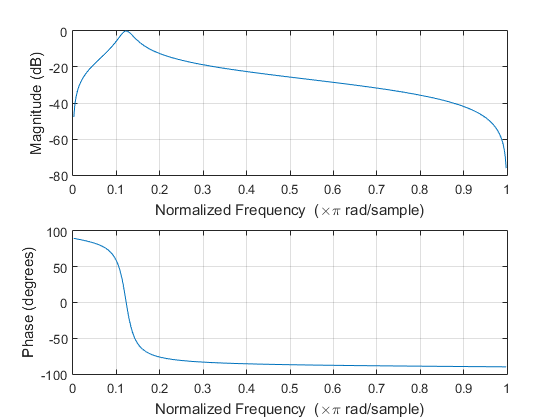
\includegraphics[width=\textwidth]{Cheby1MainFreqz}
\end{center}
\end{document}